\documentclass[pdftex,10pt,a4paper,oneside]{article}
%Can change the pt, papersize etc.

\usepackage{algorithm}
\usepackage{algorithmic} %Algorithm styles, need to be nested for the example shown
\usepackage{fancyhdr} %For our headers
\usepackage{graphicx} %Inserting images
\usepackage{lipsum}  %Blank text fill, delete me when finished
\usepackage{setspace} %Spacing on the front page for crest and titles
\usepackage[]{fncychap} % Styles can be Sonny, Lenny, Glenn, Conny, Rejne, Bjarne and Bjornstrup
\usepackage[hyphens]{url} %Deals with hyphens in urls to make them clickable
\usepackage{xcolor} %Great if you want coloured text
\usepackage{tabularx}
\usepackage{appendix} %Take a wild guess slick

%KEEP THIS ONE LAST it's quite buggy, it allows you to click on links within the pdf and web links without changing the colour. The mouse cursor simply changes its icon to indicate to the user. Great tool - still awkward
\usepackage[hidelinks]{hyperref}


%This will tell the compiler to do the header style, page and spacing between the header and text
\fancyhf{}
\renewcommand{\headrulewidth}{0.2pt}

\begin{document}

\begin{spacing}{2}
	\begin{center}
		
\includegraphics[scale = 0.20]{fwd.jpg}
	\end{center}
	\vspace{5mm}
	\begin{center}
		\textbf{\begin{LARGE}
	        Traffic Light Project
		\end{LARGE}}
		\vspace{30mm}
	\end{center}
	\begin{center}
		\textbf{\large Name: Mohamed Elesaily}
		\vspace{70mm}
	\end{center}
	\begin{center}
	     {\large NOV 2022\\}
	\end{center}
\end{spacing}

\pagebreak

\tableofcontents

\pagebreak

\section{System Description}
This project implement  Traffic light system that contain Traffic light for cars and pedestrian light for peoples. Traffic light contain green, yellow, Red lights that blinking every five seconds. 
Light blinking sequence will be:
\begin{itemize}
	\item Green blinking 5 Sec.
	\item Yellow blinking 5 Sec.
	\item Red blinking 5 Sec.
	\item Then Red, Yellow and Green.
  \end{itemize} 
pedestrian blinking sequence when pressing pedestrian button will be:
\begin{itemize}
	\item If cars' Red LED is on, the pedestrian's Green LED and the cars' Red LEDs will be on for five seconds, this means that pedestrians can cross the street while the pedestrian's Green LED is on.
	\item If Green LED is on or the cars' Yellow 
	LED is blinking, the pedestrian Red LED will be on
	 then both Yellow LEDs start to blink for five seconds, then the cars' Red LED and pedestrian Green LEDs are on for five seconds, this means that pedestrian must wait until the Green LED is on.
	\item Traffic lights signals are going to the normal mode again
  \end{itemize} 
\section{System Design}
I divide my my architecture into 5 layers (see figure \ref{s}):
\begin{figure}[H]
  \centering
  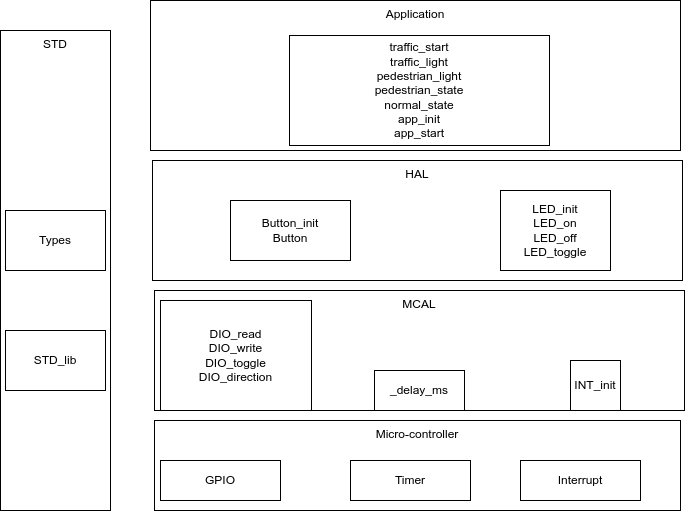
\includegraphics[width=100mm,scale=5]{architecture.png}
  \caption{Architecture}
  \label{s}
\end{figure}
 \begin{itemize}
	\item micro-controller: prephiral that used from micro-controller
	\item MCAL: drivers for prephirals
	\item HAL: drivers for Interfaces
	\item STD: shared library between all layers that have basic types and operations.
	\item Application: state machine of the traffic application
 \end{itemize}

\section{State Machine}

\begin{figure}[H]
  \centering
  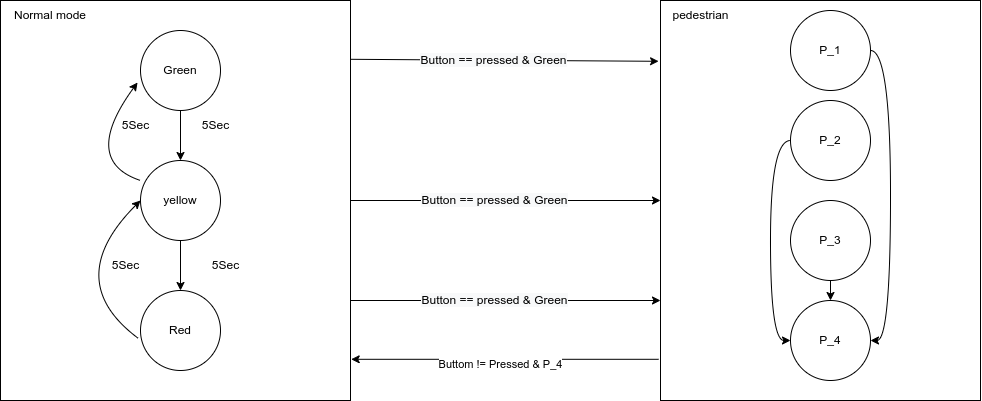
\includegraphics[width=100mm,scale=5]{state_machine.png}
  \caption{State Machine}
  \label{a}
\end{figure}
According to the requirements, I divided the states into two super states:
\begin{itemize}
	\item \textbf{Normal State}: normal state contains 3 states. Green state to blink green 
	led and after five seconds will transition to Yellow state and after five second 
	will transition to red state then vice versa
	\item \textbf{pedestrian State}: I will transition to  this state if Button is pressed and the transition will differ that depending on 
	the last state when I pressed the Button:
	\begin{itemize}
		\item if button is pressed in the Green state, app will transit to P\_2 state and by finishing the sequence will go to P\_4 state to go to normal mode.
		\item if button is pressed in the Red state, app will transit to 
		P\_1 state and by finishing the 
		sequence will go to P\_4 state to go to normal mode. 
		\item if button is pressed in the Yellow state, app will transit to 
		P\_3 state and by finishing the 
		sequence will go to P\_4 state to go to normal mode. 
	
	\end{itemize}
\end{itemize}
\end{document}
